%%%%%%%%%%%%%%%%%%%%%%%%%%%%%%%%%%%%%%%%%%%%%%%%%%%%%%%%%%%%%%%%%%%%%%%%%%%%%%%%%%
\begin{frame}[fragile]\frametitle{}
\begin{center}
{\Large PCA with Scikit-Learn}
\end{center}
\end{frame}

%%%%%%%%%%%%%%%%%%%%%%%%%%%%%%%%%%%%%%%%%%%%%%%%%%%
\begin{frame}[fragile]
\frametitle{PCA Template Code}
\begin{lstlisting}
from sklearn.decomposition import PCA

pca = PCA(n_components=4)

X = normalize(data['X'])
X_projected = pca.fit_transform(X) 
\end{lstlisting}
\end{frame}


% %%%%%%%%%%%%%%%%%%%%%%%%%%%%%%%%%%%%%%%%%%%%%%%%%%
% \begin{frame}[fragile]\frametitle{PCA}

% {\tiny (Ref: Understanding PCA - Part 2 (High-dimensional data) - Karan Rajwanshi)}


% \begin{lstlisting}
% import numpy as np
% import matplotlib.pyplot as plt
% import seaborn; seaborn.set()
% from sklearn import datasets
% from sklearn.decomposition import PCA
% import pylab as pl

% iris = datasets.load_iris()
% X, y = iris.data, iris.target

% pca = PCA(n_components=2)
% pca.fit(X)
% X_reduced = pca.transform(X)
% print("Reduced dataset shape:", X_reduced.shape)

% pl.scatter(X_reduced[:, 0], X_reduced[:, 1], c=y,
           % cmap='RdYlBu')

% print("Meaning of the 2 components:")
% for component in pca.components_:
    % print(" + ".join("%.3f x %s" % (value, name)
                     % for value, name in zip(component,
                                            % iris.feature_names)))
% \end{lstlisting}


% \end{frame}

% %%%%%%%%%%%%%%%%%%%%%%%%%%%%%%%%%%%%%%%%%%%%%%%%%%%
% \begin{frame}[fragile]\frametitle{PCA Plotting}
% \begin{center}
% 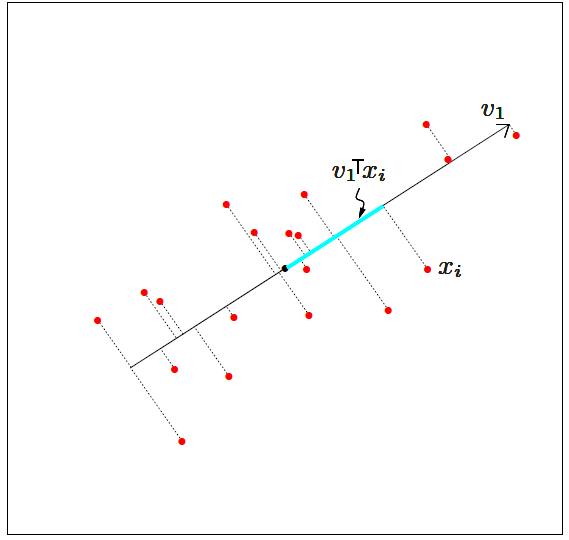
\includegraphics[width=0.8\linewidth,keepaspectratio]{pca1}
% \end{center}

% {\tiny (Ref: Understanding PCA - Part 2 (High-dimensional data) - Karan Rajwanshi)}

% \end{frame}




%%%%%%%%%%%%%%%%%%%%%%%%%%%%%%%%%%%%%%%%%%%%%%%%%%%
\begin{frame}[fragile]
\frametitle{Principal Component Analysis (Recap)}
\begin{itemize}
	\item Scikit-learn has methods to compute PCA and several variants. 
	\item Classic PCA (sklearn.decomposition.PCA) is based on an eigenvalue decomposition of the data co-variance, so that for N points, the computational cost grows as
	$\mathcal{O[N^3]}$. This means that for large data-sets like the current one, the fit can be very slow. 
\end{itemize}
\end{frame}

%%%%%%%%%%%%%%%%%%%%%%%%%%%%%%%%%%%%%%%%%%%%%%%%%%%
\begin{frame}[fragile]\frametitle{Alternate method}

\begin{itemize}
\item Fortunately, Scikit-learn has an alternative method that is much faster. 
\item The speed comes at a price: it is based on random projections, so the results are not as robust as the normal method. 
\item But for tasks such as ours where we are seeking only a few of a large number of eigen-vectors, it performs fairly well. 
\item To keep our results consistent between runs, we'll explicitly set the random seed for the fit. 
\item You should repeat this with several different random seeds to convince yourself that the results are consistent:
\end{itemize}
\end{frame}


%%%%%%%%%%%%%%%%%%%%%%%%%%%%%%%%%%%%%%%%%%%%%%%%%%%
\begin{frame}[fragile]\frametitle{Alternate method}

Linear dimensional reduction using \textit{Singular Value Decomposition} of the data and keeping only the most significant singular vectors to project the data to a lower dimensional space.

\begin{lstlisting}
from sklearn.decomposition import RandomizedPCA

rpca = RandomizedPCA(n_components=4, random_state=0)

X_proj = rpca.fit_transform(X)

X_proj.shape
(4000, 4)
\end{lstlisting}


\end{frame}

%%%%%%%%%%%%%%%%%%%%%%%%%%%%%%%%%%%%%%%%%%%%%%%%%%%%%%%%%%%%%%%%%%%%%%%%%%%%%%%%%%
\begin{frame}[fragile]\frametitle{}
\begin{center}
{\Large Test case: Iris Flowers}
\end{center}
\end{frame}

%%%%%%%%%%%%%%%%%%%%%%%%%%%%%%%%%%%%%%%%%%%%%%%%%%%
\begin{frame}[fragile]\frametitle{Iris: Dimensionality Reduction: PCA: Data}
\begin{lstlisting}
import numpy as np
import matplotlib.pyplot as plt
import seaborn; 
from sklearn import neighbors, datasets

import pylab as pl

seaborn.set()

iris = datasets.load_iris()

X, y = iris.data, iris.target
from sklearn.decomposition import PCA
pca = PCA(n_components=2)
pca.fit(X)
X_reduced = pca.transform(X)
print("Reduced dataset shape:", X_reduced.shape)
\end{lstlisting}
\end{frame}

%%%%%%%%%%%%%%%%%%%%%%%%%%%%%%%%%%%%%%%%%%%%%%%%%%%
\begin{frame}[fragile]\frametitle{Iris: Dimensionality Reduction: PCA: Plot}

\begin{center}
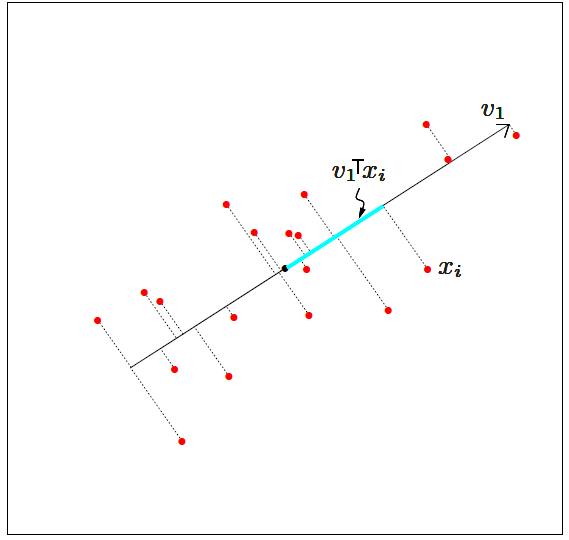
\includegraphics[width=0.4\linewidth,keepaspectratio]{pca1}
\end{center}


\begin{lstlisting}
import pylab as pl
pl.scatter(X_reduced[:, 0], X_reduced[:, 1], c=y,
           cmap='RdYlBu')

print("Meaning of the 2 components:")
for component in pca.components_:
    print(" + ".join("%.3f x %s" % (value, name)
                     for value, name in zip(component,
                                            iris.feature_names)))
\end{lstlisting}

\end{frame}

%%%%%%%%%%%%%%%%%%%%%%%%%%%%%%%%%%%%%%%%%%%%%%%%%%%%%%%%%%%%%%%%%%%%%%%%%%%%%%%%%
\begin{frame}[fragile]\frametitle{}
\begin{center}
{\Large Can you write PCA from Scratch? hmm, using numpy}
\end{center}
\end{frame}

%%%%%%%%%%%%%%%%%%%%%%%%%%%%%%%%%%%%%%%%%%%%%%%%%%%
\begin{frame}[fragile]\frametitle{PCA: Exercise}
Load Data
\begin{lstlisting}
data = loadmat('data/ex7data1.mat')
X = data['X']
fig, ax = plt.subplots(figsize=(12,8))
ax.scatter(X[:, 0], X[:, 1])
\end{lstlisting}
\begin{center}
\includegraphics[width=0.5\linewidth,keepaspectratio]{pca17}
\end{center}
\end{frame}

%%%%%%%%%%%%%%%%%%%%%%%%%%%%%%%%%%%%%%%%%%%%%%%%%%%
\begin{frame}[fragile]\frametitle{PCA: Stubs}
 After ensuring that the data is normalized, the output is simply the singular value decomposition of the co-variance matrix of the original data.
\begin{lstlisting}
def pca(X):
    # normalize the features
    X = (X - X.mean()) / X.std()
    
    # compute the covariance matrix
    X = np.matrix(X)
    cov = (X.T * X) / X.shape[0]
    
    # perform SVD
    U, S, V = np.linalg.svd(cov)
    
    return U, S, V
\end{lstlisting}
\end{frame}

%%%%%%%%%%%%%%%%%%%%%%%%%%%%%%%%%%%%%%%%%%%%%%%%%%%
\begin{frame}[fragile]\frametitle{PCA: Exercise}
\begin{lstlisting}
U, S, V = pca(X)    

matrix([[-0.79241747, -0.60997914],
         [-0.60997914,  0.79241747]]),
 array([ 1.43584536,  0.56415464]),
 matrix([[-0.79241747, -0.60997914],
         [-0.60997914,  0.79241747]]))
\end{lstlisting}
\end{frame}


%%%%%%%%%%%%%%%%%%%%%%%%%%%%%%%%%%%%%%%%%%%%%%%%%%%
\begin{frame}[fragile]\frametitle{PCA: Exercise}
Now that we have the principal components (matrix U), we can use these to project the original data into a lower-dimensional space. 
\begin{lstlisting}
def project_data(X, U, k):
    U_reduced = U[:,:k]
    return np.dot(X, U_reduced)

Z = project_data(X, U, 1)
\end{lstlisting}
\end{frame}

%%%%%%%%%%%%%%%%%%%%%%%%%%%%%%%%%%%%%%%%%%%%%%%%%%%
\begin{frame}[fragile]\frametitle{PCA: Exercise}
We can also attempt to recover the original data by reversing the steps we took to project it.
\begin{lstlisting}
def recover_data(Z, U, k):
    U_reduced = U[:,:k]
    return np.dot(Z, U_reduced.T)
    
X_recovered = recover_data(Z, U, 1)
fig, ax = plt.subplots(figsize=(12,8))
ax.scatter(X_recovered[:, 0], X_recovered[:, 1])
\end{lstlisting}
\end{frame}

%%%%%%%%%%%%%%%%%%%%%%%%%%%%%%%%%%%%%%%%%%%%%%%%%%%
\begin{frame}[fragile]\frametitle{PCA: Exercise}
\begin{center}
\includegraphics[width=0.5\linewidth,keepaspectratio]{pca18}
\end{center}
\begin{itemize}
\item Notice that the projection axis for the first principal component was basically a diagonal line through the data set. 
\item When we reduced the data to one dimension, we lost the variations around that diagonal line, so in our reproduction everything falls along that diagonal.
\end{itemize}
\end{frame}

%%%%%%%%%%%%%%%%%%%%%%%%%%%%%%%%%%%%%%%%%%%%%%%%%%%%
%\begin{frame}[fragile]\frametitle{Parameters}
%\begin{itemize}
%\item n\_components : int, None or string
%Number of components to keep. if n\_components is not set all components are kept:
%n\_components == min(n\_samples, n\_features)
%if n\_components == `mle', Minka's MLE is used to guess the dimension if $0 < n\_components < 1$, select the number of components such that the amount of variance that needs to be explained is greater than the percentage specified by n\_components
%\item copy : bool
%If False, data passed to fit are overwritten and running fit(X).transform(X) will not yield the expected results, use fit\_transform(X) instead.
%\item whiten : bool, optional
%When True (False by default) the components\_ vectors are divided by n\_samples times singular values to ensure uncorrelated outputs with unit component-wise variances.
%\end{itemize}
%\end{frame}
%
%%%%%%%%%%%%%%%%%%%%%%%%%%%%%%%%%%%%%%%%%%%%%%%%%%%%
%\begin{frame}[fragile]\frametitle{Whitening}
%Whitening will remove some information from the transformed signal (the relative variance scales of the components) but can sometime improve the predictive accuracy of the downstream estimators by making there data respect some hard-wired assumptions. Attributes:
%\begin{itemize}
%\item components\_ : array, [n\_components, n\_features]
%Components with maximum variance.
%\item explained\_variance\_ratio\_ : array, [n\_components]
%Percentage of variance explained by each of the selected components. k is not set then all components are stored and the sum of explained variances is equal to 1.0
%\item mean\_ : array, [n\_features]
%Per-feature empirical mean, estimated from the training set.
%\item n\_components\_ : int
%The estimated number of components. Relevant when n\_components is set to ‘mle' or a number between 0 and 1 to select using explained variance.
%\item noise\_variance\_ : float
%\end{itemize}
%\end{frame}
